
There are several metrics that can be used for comparison of the different 
delay models and parameters. They can be divided into two types: Power 
comparison and waveform comparison. In the following, both types are described.

\subsection{Power comparison}
\label{sec:man-evaluation-power-comparison}
The \spice\ simulation performs two different power estimations - the average 
power consumption and the maximum power consumption.

\subsubsection{Average power consumption}
For the average based power consumption, two types of reference values are 
used. The first one is the estimation by the \spice\ simulation 
(\spice/\spice), and the second 
one is the power estimation by \dc\ and \primetime\, based on the trace of 
\spice\ simulation (\spice/column). Using these two types of reference values 
is helpful for distinguishing deviations because of different tools and 
deviations because of different delay models. In general, the two types of 
reference values should be similar ($\pm \SI{5}{\percent}$). 
Using a \file{*.spef} file for the power estimation with \dc\ and \primetime\ 
increases the accuracy of these tools, and therefore in general reduces the 
deviation to the \spice\ reference.

\subsubsection{Maximum power consumption}
\label{sec:man-evaluation-maximum-power-consumption}
The time-based power estimation method of \primetime\ can also estimate the 
maximum power consumption. This result can be compared to the estimation of the 
\spice\ simulation, but unfortunately the results can differ significantly, and 
therefore this metric was discarded.

\subsection{Waveform comparison}
\label{sec:man-evaluation-waveform-comparison}

During the reporting process, the resulting traces of the \modelsim\ simulation 
with the standard delay model and the involution delay model are compared to 
the \spice\ trace, which is used as reference. In the following sections, the 
different metrics that are based on the waveforms are described.

\subsubsection{Number of transitions}
One of the simplest metrics is to sum up the number of transitions on each 
trace and compare them. The \invt\ also calculates the maximum deviation on a 
single signal, in order to find out the part of the circuit, where the 
deviation is the most. 

\subsubsection{Area under the deviation trace}
For the deviation trace, the absolute value of the difference between a trace 
(\modelsim\ or Involution delay model) and the \spice\ reference trace is 
calculated. The area under the deviation trace is calculated by multiplying the 
duration of the deviation with the value of the deviation ($V_{DD}$).
A more sophisticated approach is to find corresponding transitions on both 
compared traces, and calculated the signed area of the deviation. The area is 
counted positive if the compared trace is leading against the \spice\ trace, 
otherwise the area is counted negative. This metric can help to find problems 
in the \sdffile, for example if the delays are to long in general, the negative 
area is significantly larger than the positive area.

\subsubsection{Glitches}
The \invt\ also counts the number of glitches. Several types can be 
distinguished:

\begin{itemize}
	\item Type of glitch:
	\begin{itemize}
		\item original (o): This is what is in general considered as typical 
		glitch. Both signals are on the same level, then two subsequent 
		transitions happen on one of the two signals.
		\item inverted (i): Both signals are one opposite levels, then two 
		subsequent transitions happen on one signal, and after these two 
		transitions they are again on different levels.
	\end{itemize}
	\item Location of glitch:
	\begin{itemize}
		\item induced (i): If the glitch is on the trace of the digital delay 
		model. Compared to the \spice\ reference, a glitch has been induced.
		\item suppressed (s): Two subsequent transitions happen on the \spice\ 
		reference signal, and these two transitions are not made by the 
		simulation with the digital delay model.
	\end{itemize}
	
\end{itemize}

Two subsequent transitions on one trace without a transition on the other trace 
are called glitch. Figure~\ref{fig:man-inv_tool_glitches} shows all four 
combinations of glitches according to the classification above. The first 
character denotes the type of the glitch, the second the location of the glitch.
Figure~\ref{fig:man-inv_tool_glitches} also shows how the deviation trace for 
two arbitrary traces looks like.

\begin{figure}[!ht]
	\centering
	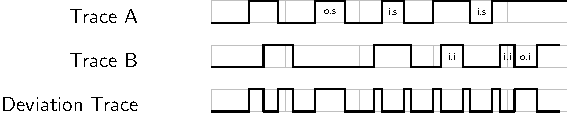
\includegraphics[width=0.9\textwidth]{figures/glitches.pdf}
	\caption{Types of glitches.}
	\label{fig:man-inv_tool_glitches}
\end{figure}

Note that for better comparability between different circuits, the number of 
glitches can be divided by overall number of transitions. 
We decided to use for the induced glitches the number of transitions on the 
corresponding \modelsim\ / Involution delay model trace, and for the suppressed 
glitches the number of transitions on the reference signal. 
This process is currently performed manually on the resulting 
\file{results.csv} file of the \multiexec\ tool. 
The plotting tool (Section~\ref{sec:man-plots}) already supports these glitch 
percentage values.

\subsubsection{Leading / Trailing against reference}

The leading / trailing metrics aim at mapping the area under deviation and the 
number of transitions to an average value how soon or late transitions take 
place, compared to the \spice\ reference. Note that these metrics are not 
directly calculated by the \invt, but all the required values are extracted by 
the tool and therefore they can be easily calculated during the post 
processing. The plotting tool described in Section~\ref{sec:man-plots} already 
supports these metrics. Nevertheless the preparation for the plotting tool is 
still performed manually (as described in Section~\ref{sec:man-plots}).

They come in three different flavors:
\begin{itemize}
 	\item the positive / negative area under the deviation trace divided by the 
 	number of transitions on the \spice\ reference.
 	\item the positive / negative area under the deviation trace  divided by 
 	the number of transitions where the trace was leading / trailing compared 
 	to the \spice\ reference.
 	\item same as previous, but only transitions which are no glitch are 
 	considered.
\end{itemize}

\subsubsection{Remarks}

Note that the described metrics are by far not complete, and that these are 
only the ones we considered most important during the development process. Due 
to the structure of the \invt, extracting more values and adding new metrics 
should be easy. Moreover, for different task other metrics might be more 
suitable.